%%% LITERATURE REVIEW
\addcontentsline{toc}{section}{Abstract}
\section*{Abstract}
Traits are fundamental characteristics, measurable at the level of an individual, that impact organismal fitness and performance. Traits that influence how species respond to environmental changes have been termed `response' traits, as opposed to `effect' traits, that shape ecosystem processes. As such, traits can provide with (1) a mechanistic link between environmental change and species responses; (2) a mechanistic link between community composition and ecosystem functioning. 

Here, I summarise the current empirical evidence that has been gathered in identifying response traits to climate and land-use change in terrestrial vertebrates. Studies mostly focused on a subset of vertebrate classes and were most often conducted at local or regional scales. As such, whether response traits that have been identified can be generalised geographically and taxonomically remains to be largely explored, emphasising the need for global scale comparative studies. 

The trait composition of ecological communities is often summarised using functional diversity indices. In animal communities, functional diversity indices do not correlate well with ecosystem functioning, partly because a single ecosystem process can arise from a combination of traits that can be difficult to capture. Despite many studies documenting how anthropogenic threats reshape the functional composition of local vertebrate communities, our understanding of how human pressures will impact the processes vertebrate species sustain remains limited. 

The work in the present report focuses on compiling trait data for terrestrial vertebrates, and investigating how land-use change alters the functional composition of local communities. Hypotheses are presented at the end of this Chapter, and detailed further in each corresponding Chapter.

\section{Land-use and climate change, species traits and the functional composition of vertebrate communities}

\subsection{Land-use and climate change and species response traits}

Currently, terrestrial land-use change is the most important driver of biodiversity declines \citep{Newbold2015, Chaudhary2016, Maxwell2016}.  With climate change projected to be catching up by 2070 \citep{Newbold2018}, it has become vital to understand how these threats will affect biodiversity, separately and in combination. By influencing species responses to environmental changes, response traits can provide a mechanistic understanding of how diverse threats shape ecological communities, an understanding particularly relevant for conservation policies. 

There is now empirical evidence across taxonomic groups that species traits influence their responses to LUCC. For instance, response traits to LUCC have been identified in terrestrial plant \citep{Diaz2001}, fungal \citep{Koide2013}, invertebrate \citep{Williams2010, Hall2019}, and terrestrial vertebrate species (Table \ref{referencestable}).
It is important to point out that in some cases, contrasting results are found (for instance, in bees: larger body size having been found to influence species responses to land-use change both negatively \citep{Larsen2005} and positively \citep{Depalma2015}, or having been found to have little effect \citep{Williams2010, Forrest2015}, see \citet{Bartomeus2018}). This highlights the fact that studies may be context-dependent, with contingent limitations. For vertebrates, most studies, conducted on different taxa and at different scales, tend to show that larger, longer-lived specialist species with a lower reproductive output are more likely to be impacted negatively by LUCC (Table \ref{referencestable}). As such, a number of response traits to land-use or climate change have been identified for vertebrate species belonging to diverse classes (Table \ref{referencestable}).

Despite this empirical evidence, there is still a need to refine our understanding of which traits significantly influence responses. As traits are commonly used to assess species vulnerability to threats or extinction risks \citep{Pacifici2015, Willis2015,Bohm2016b}, it is particularly important to be confident about how they act on species responses. Trait-based approaches can be opposed to trend-based approaches \citep{Pacifici2015}, which rely on historic population trends (changes in abundance or shifts in distributions) to predict species vulnerability and extinction risks. Trend-based approaches require important field work effort to monitor species populations. Getting extensive information on all species population trends is virtually impossible. The appeal of trait-based approaches is that, by providing mechanistic insights, they diminish the amount of population information needed. If species' responses to a threat consistently relate to certain traits, it is possible to generalise patterns across species for which data is less available \citep{Verberk2013}. Nevertheless, for several reasons that I now expose, how species traits influence their responses to LUCC remains unclear.

First, there is a lack of comprehensive understanding about which traits are important in shaping species responses to climate change. \citet{Wheatley2017} compared different published climate change vulnerability assessment frameworks, some of which trait-based, some trend-based, and some incorporating elements of both (hybrid). They found that the different frameworks, applied to the same set of species, did not yield consensual outputs and classified species inconsistently into different risk categories. Their work underlines that currently, trend-based vulnerability assessments perform better at identifying species at risks from climate change than trait-based approaches. This study highlights the current lack of unanimous understanding as to which traits to consider, and how, in vulnerability assessments. More broadly, their study stresses the need to clarify our understanding of how response traits to climate change act across different taxa. The finding in \citet{Wheatley2017} that there is no consensus across assessment frameworks might be explained by the fact that frameworks were initially designed and tested for a particular taxon -- generally at the class level or lower ranks --, and do not hold when applied to other taxa. They nevertheless argue that frameworks should be universally applicable. Their findings put into question to our current ability to extrapolate the knowledge of response traits gathered for certain taxa to other taxonomic groups. 


\begin{landscape}
\begin{table}[]
\begin{center}\fontsize{9}{11}\selectfont
\renewcommand{\baselinestretch}{1}
\renewcommand{\arraystretch}{1}
\caption{Some references providing with empirical evidence for response traits to LUCC in terrestrial vertebrates. Also see \citet{Hevia2017}.}
%The directionality of the effect is indicated with a + (when higher trait values or higher degrees of specialisation confer more sensitivity to a pressure) or a - (in the opposite case).
\label{referencestable}
\begin{tabular}{lllll}
\hline
\multicolumn{1}{c}{\textbf{Pressure}}                                                                                       & \multicolumn{1}{c}{\textbf{Reference}}                                                     & \multicolumn{1}{c}{\textbf{Trait or property}}                                                                                                                                                             & \multicolumn{1}{c}{\textbf{Taxa}}                               & \multicolumn{1}{c}{\textbf{Study scale}}                                      \\ \hline
Land-use change                                                                                                             & \citet{Newbold2013} & \begin{tabular}[c]{@{}l@{}}Generation length \\   Body mass \\   Migratory activity\\   Diet specialisation \\   Habitat specialisation \end{tabular}                                          & Birds                                                           & Pan-tropical forests                                                          \\ \hline
Urbanisation                                                                                                                & \citet{LaSorte2018}                                                                      & \begin{tabular}[c]{@{}l@{}}Body mass\\   Range size\\   Diet specialisation\\   Foraging strata\\   Habitat specialisation\end{tabular}                                                         & Birds                                                           & Global (58 cities)                                                            \\ \hline
Habitat modification                                                                                                        & \citet{Nowakowski2017} & \begin{tabular}[c]{@{}l@{}}Range size\\   Habitat specialisation\end{tabular}                                                                                                                              & Amphibians                                                      & Global                                                                        \\ \hline
Land-use change                                                                                                             & \citet{Flynn2009} & \begin{tabular}[c]{@{}l@{}}Litter size (Mammals)\\   Diet (Mammals)\\   Body mass (Birds)\\   Diet (Birds)\\   Foraging habits (Birds)\end{tabular}                                                        & \begin{tabular}[c]{@{}l@{}}Mammals\\   Birds\end{tabular}       & America                                                                       \\ \hline
\begin{tabular}[c]{@{}l@{}}Human pressure history \\ (human population density and \\ land-conversion history)\end{tabular} & \citet{Rapacciuolo2017} & Body mass                                                                                                                                                                                                  & Tetrapods                                                       & Western Hemisphere                                                            \\ \hline
Land-use change                                                                                                             & \citet{Tinoco2018}             & Body mass                                                                                                                                                                                                  & Hummingbirds                                                    & \begin{tabular}[c]{@{}l@{}}Andes Mountains, southern\\   Ecuador\end{tabular} \\ \hline
Habitat loss                                                                                                                & \citet{Quesnelle2014} & Reproductive rate                                                                                                                                                                                          & Wetland vertebrates                                             & Global                                                                        \\ \hline
\begin{tabular}[c]{@{}l@{}}Climate change \\ (Range filling proxy)\end{tabular}                                             & \citet{Estrada2018} & \begin{tabular}[c]{@{}l@{}}Habitat specialisation (Mammals)\\   Sexual maturity age (Mammals)\\   Habitat specialisation (Birds)\\   Reproductive output (Birds)\end{tabular}                              & \begin{tabular}[c]{@{}l@{}}Mammals\\   Birds\end{tabular}       & Europe                                                                        \\ \hline
Climate change                                                                                                              & \citet{Pacifici2017} & \begin{tabular}[c]{@{}l@{}}Habitat specialisation (Mammals)\\   Diet (Mammals)\\   Dispersal abilities (Birds)\\   Generation length (Birds)\\   Altitudinal range\\   (non-breeding) (Birds)\end{tabular} & \begin{tabular}[c]{@{}l@{}}Mammals\\   Birds\end{tabular}       & Global                                                                        \\ \hline
Climate change                                                                                                              & \citet{Pearson2014}                                                                       & \begin{tabular}[c]{@{}l@{}}Occupied area\\   Generation length\\   Operational thermal range\end{tabular}                                                                                                  & \begin{tabular}[c]{@{}l@{}}Amphibians\\   Reptiles\end{tabular} & USA                                                                           \\ \hline
Climate change                                                                                                              & \citet{Mccain2014} & \begin{tabular}[c]{@{}l@{}}Body mass\\   Activity time\end{tabular}                                                                                                                                        & Mammals                                                         & North America                                                                 \\ \hline
Climate change                                                                                                              & \citet{Schloss2012}                & Dispersal ability                                                                                                                                                                                          & Mammals                                                         & Western Hemisphere                                                            \\ \hline
Climate change                                                                                                              & \citet{Angert2011}                                                                                & \begin{tabular}[c]{@{}l@{}}Diet breadth \\   Migratory status\\   Reliance on open water\end{tabular}                                                                                                   & Birds (Passeriformes)                                           & North America                                                                 \\ \hline
\end{tabular}
\end{center}
\end{table}

\end{landscape}





To my knowledge, comparative studies looking at whether response traits to LUCC differ across taxonomic groups (at ranks higher than class), experiencing the same threat levels under similar conditions, are rare. The picture becomes even more complex when different studies find contradicting results within a taxon, such as was the case in some bee species \citep{Bartomeus2018}. Moreover, the importance of response traits may vary geographically. The work by \citet{Bartomeus2018} further emphasises the idea that unless similar response traits to a threat are identified consistently across different systems and taxa, our ability to use traits as predictors of vulnerability or extinction risk remains limited. For these reasons, it is necessary to conduct comparative analyses across taxa, to identify response traits, verify whether they are conserved across species and whether they have the same importance in shaping responses across taxonomic groups and geographical areas. 

Second, another difficulty when identifying response traits is that different threats can be acting on the studied ecological community, so that observed modifications stem from the interactions of diverse response traits \citep{Gonzalez-Suarez2013}. Response traits must be identified for a single threat while controlling for others, before investigating potential interacting effects. Nevertheless, this is difficult to achieve when using global empirical data.  For land-use change, this difficulty can be overcome by using data collected over sufficiently small-scale areas, over which other pressures can be assumed to be negligible. 

To conclude, potential taxon-, threat- and geographical dependence of response traits to land-use or climate change makes it difficult to generalise patterns observed at local scales. This stresses the need to conduct global, cross-taxon studies to verify whether empirical evidence supports the generalisation of any response trait. Identifying response traits using global scale data, across the four terrestrial vertebrate classes, is one the goal of my PhD project.

\subsection{Land-use and climate change, functional diversity and the disruption of ecosystem services}

Response traits allow to understand and predict how environmental pressures are likely to modify ecological assemblages (changes in species richness and abundance). These alterations can lead to modifications in functional diversity (the diversity and variability of functional traits  in a community). Several indices have been developed in the recent years to estimate diverse components of functional diversity \citep{Schleuter2010, Villeger2008, Legras2018, Laliberte2010}. Functional diversity indices are interesting for at least two reasons. First, they can inform on how disturbances affect trait community composition. Second, as functional (effect) traits relate to ecosystem functions, measures of functional diversity are often used as a proxy for ecosystem functioning. I will develop these two points in more detail further down, and I will mainly focus on land-use change as the disturbance of interest. 

\paragraph{Impacts of land-use change on the functional diversity of vertebrate communities.}

Response traits determine whether a species is likely to be removed from a community due to the environmental filtering exerted by a pressure such as land-use change. Environment filtering is a major driver of community structure (but see \citet{Cadotte2017}); it refers to a process whereby environmental conditions select out species that cannot get established and cannot persist in a given area. As environmental filtering imposes barriers on establishment and survival, it is expected that species with similar traits, which render them able to persist in the altered conditions, are favoured \citep{Wong2018, Cadotte2017}. Consequently, the trait composition of emergent communities is expected to be non-randomly impacted.  The trait composition of a community can be assessed in different ways. When dealing with individual traits separately, community-weighted means are often employed. Trait distributions can also be compared across a land-use gradient. Finally, functional diversity indices allow to consider several traits simultaneously. As such, they provide with estimates summarising multivariate trait composition.

Various indices have been developed in the past years to estimate different facets of functional diversity. They have notably been reviewed in \citet{Schleuter2010} and in \citet{Legras2018}. Some indices are, by construction, independent from species richness, while others are known to covary with species richness \citep{Schleuter2010}. Here, I will present two indices aiming at estimating the functional richness of ecological communities, as well as two indices quantifying multivariate trait dispersion.

\subparagraph{Functional richness.} 
Functional richness was initially assessed by grouping species together into functional groups: species sharing similar trait values were assumed to belong to the same functional group. Functional richness was then assessed as the total number of functional groups \citep{Legras2018}. As underlined by \citet{Legras2018}, this approach is problematic for several reasons: the definition of functional groups depends on users' choices, notably to define trait boundaries between groups, which is particularly problematic with continuous traits. Consequently, other indices have been developed to estimate functional richness; in this work, I focus on two indices, which rely two different conceptual bases. These indices will be described in more details in Chapter 3 (see Figure \ref{chartFR_calc} in Chapter 3).

\paragraph{FRic \citep{Villeger2008}.}
The FRic index, developed by \citet{Villeger2008}, aims at estimating the amount of trait space that species occupy. This index relies on the projection of species in a multidimensional space, where each dimension is a trait (or a principal component, if the dimensionality of the trait dataset has been reduced). Species are placed in the multidimensional space according to their trait values. The functional richness is then estimated as the volume of the convex hull that encompasses all species of a given community \citep{Villeger2008}.
  
\paragraph{DFR (denominated `FD' by \citet{Petchey2002}).}
The dendrogram-based functional richness index developed by \citet{Petchey2002} aims at estimating the total functional distance among species of a given community. Its calculation relies on the obtention of a functional dendrogram, from which functional richness is estimated as the sum of branch lengths for the species in a given community. The functional dendrogram is obtained by clustering a species$\times$species distance matrix, derived from a species$\times$trait dataset. In this work, dendrogram-based functional richness is referred to as DFR. DFR has notably been criticised for being sensitive to the choice of the clustering method \citep{Legras2018}.
 
\vspace{0.5cm}
Both FRic and DFR are conceptually, by construction, not independent from species richness. In experimental studies and natural communities, a positive correlation between functional and species richness is often found \citep{Cadotte2011}. For this reason, examining whether functional richness indices inform on community dynamics differently from species richness is an important question to elucidate. Indeed, if species richness is as informative as functional richness, the latter is not worth measuring: species richness is then a proxy for functional richness. This question was central to the study conducted by \citet{Cadotte2011}. By reviewing the literature, they found that the relationship between functional richness and species richness is context-dependent, and that the shape of the relationship notably depends on the amount of functional redundancy in the community. 

Functional redundancy aims at describing the degree to which species in a given assemblage share similar trait values, and, as such, sustain similar ecosystem processes \citep{Mayfield2010, Rosenfeld2002, Ricotta2016}. In communities with a high degree of functional redundancy, functions can be maintained despite species loss. On the other hand, the loss or gain of functionally diverse species can lead to marked variations in functional richness, despite small changes in species richness (Figure \ref{fredundancy_ltr}). Furthermore, \citet{Mayfield2010} showed that the relationship between species richness and functional richness could be affected in different ways by human land-uses. They proposed diverse mechanisms building upon community assembly processes to explain how land-uses may influence species richness -- functional richness trajectories.  

\begin{figure}[h!]
\centering
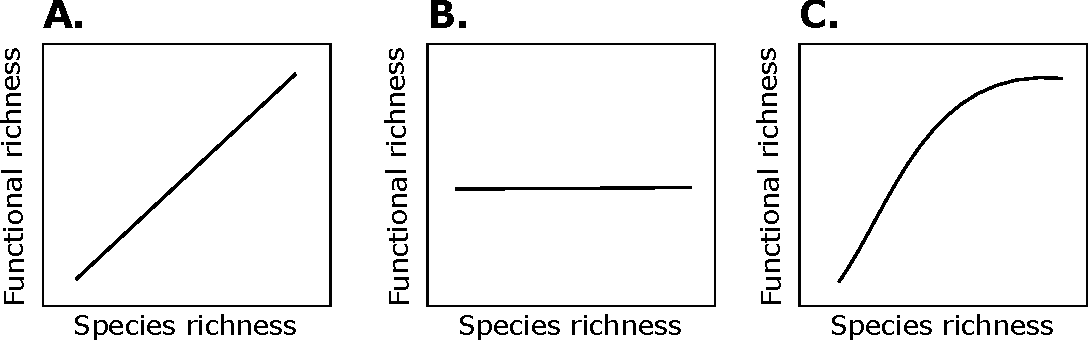
\includegraphics[scale=0.7]{figures/chapter1/Fredundancy.pdf}
\caption[The species richness -- functional richness relationship informs on functional redundancy.]{\textbf{The species richness -- functional richness relationship informs on functional redundancy.} \textbf{(A)} High positive correlation between species richness and functional richness: functional richness increases at a constant rate with species richness. The gain or loss of species can lead to marked variations in functional richness. The rate of increase is higher than in \textbf{(B)}, where functional richness remains constant despite variations in species richness. The functional redundancy of \textbf{(B)} is comparatively higher than that of \textbf{(A)}. \textbf{(C)} The rate at which functional richness increases with increases in species richness is not constant. The functional redundancy increases with higher species richness.} 
\label{fredundancy_ltr}
\end{figure}

The potential correlation of species richness with functional richness has two practical consequences. 

First, as underlined above, the shape of the relationship can inform on the functional redundancy of a given community (\cite{Cadotte2011}, and Figure \ref{fredundancy_ltr}). Thus, changes in the relationship between functional richness and species richness across a land-use gradient can provide insights into how land-use change impacts the functional redundancy of ecological communities. In assemblages with functionally redundant species, random species loss or addition are unlikely to lead to marked variation in functional richness.

Second, when species richness strongly correlates with functional richness (Figure \ref{fredundancy_ltr} A), decreases in functional richness along a land-use gradient may be due to decreases in species richness alone. In other words, an observed change in functional richness may be driven by changes in species richness alone rather than by environmental filtering. As such, it becomes necessary to disentangle the effects of species richness from the effects of the environmental variable of interest. To that end, a common approach consists in generating the null expectation of functional richness given a species richness. Then, empirical values can be compared against null expectations. This can be achieved through simulations where the community composition is randomised, given a species richness, so as to generate a null distribution of functional richness \citep{Wong2018, Flynn2009}.

\subparagraph{Functional dispersion.}
When a community is subject to environmental filtering, functional clustering is expected to be observed in the emergent community \citep{Wong2018, Cadotte2017}. Functional clustering -- also referred to as functional under-dispersion -- qualifies communities where species are more similar, in term of their traits, than expected by chance. Diverse indices have been developed to quantify the functional dispersion of ecological communities (for instance, Rao's quadratic entropy, or functional dispersion FDis, developed by \citet{Laliberte2010}). Rao's quadratic entropy and FDis aim at assessing the degree to which species resemble each other in terms of their traits. Chapter 3 provides more details on their definition and calculation (see Figure \ref{chartFDis}). 

Rao's quadratic entropy and functional dispersion are highly correlated. Both can be used to assess whether species in a given community are functionally clustered, as a consequence of environmental filtering. For instance, the observed dispersion in trait values can be compared to the null expectation of functional dispersion, obtained from a null model. As these indices are, by construction, independent from species richness, the effects of environmental filtering on functional dispersion can also be deduced directly from shifts in the values of the indices along an environmental gradient. 

As anthropogenic land-uses globally negatively impact local species richness \citep{Newbold2015}, decreases in functional richness of local ecological communities are likely to take place, particularly in communities with low functional redundancy. Moreover, land-use change could also alter the functional richness of communities without altering local species richness. For instance, \citet{Flynn2009} showed that the functional richness (DFR) of avian, mammalian and plant communities located in the Western hemisphere decreased under agricultural intensification. \citet{Chapman2018} showed that the functional richness (DFR) of tropical bird communities declined along a land-use gradient of increasing human disturbance. Other studies have reported shifts in the distribution of trait values along land-use gradients \citep{LaSorte2018, Rapacciuolo2017}. Overall, all these studies show that land-use change alters the functional richness of local vertebrate assemblages. Nevertheless, most studies were conducted at local or regional scales.

Some studies have been conducted at global scales to understand patterns in the functional dispersion of avian assemblages \citep{Cooke2019}, or in the functional richness (DFR) of mammalian communities \citep{Safi2011}. Nevertheless such studies did not focus on land-use change or other anthropogenic pressures, but on latitudinal gradients of species diversity. As such, to my knowledge, no study has yet investigated how land-use change impacts the functional diversity of local vertebrate communities at global scales. 

Studies looking at the effects of climate change on the functional diversity of terrestrial vertebrates are also rare. \citet{BarbetMassin2015} investigated how future climate change was projected to impact the functional diversity of global avian assemblages through range shifts. \citet{Thuiller2014} investigated how both projected land-use and climate change affected the functional diversity of European avian assemblages. Both studies highlighted that future range shifts due to climate change leaded to uneven effects on functional diversity across space, with some areas projected to experience substantial loss of functional diversity. To my knowledge, no work has investigated how future climate change is likely to impact the functional diversity of other vertebrate taxa (herptiles or mammals) at global scales. 

To summarise, past empirical evidence has shown that (1) species sensitivity to LUCC depends on their traits; (2) LUCC  is reshaping the functional composition of ecological assemblages, potentially disrupting important functions. Nevertheless, most studies have been conducted at local or regional scales, so that it is still unknown how global changes affect the functional diversity of local terrestrial vertebrate communities. Tackling this question, with land-use change at the disturbance of interest, is the aim of Chapter 3. 

The recent development of many functional diversity indices, synthesising the diversity of functions in a community, reflects the importance of understanding how anthropogenic pressures are likely to modify ecosystem processes. In the field of biodiversity-ecosystem functioning relationships, it is now well established that higher species diversity is associated with higher ecosystem productivity and stability, better use of limiting resource, as well as better resistance to biological invasions \citep{Tilman2014}. I now explore the links between functional diversity indices and ecosystem functioning in more details.

\paragraph{Functional diversity and ecosystem functioning}

Early experiments investigating the relationships between functional composition and ecosystem functioning classified species in broad functional groups. Species belonging to similar groups were assumed to have similar effects on ecosystem processes \citep{Legras2018}. Ecosystem functioning was measured in various ways, depending on the studied system. For instance, plant biomass was used to measure primary productivity in \citet{Weisser2017}. The field, overall, was dominated by experiments conducted on plant communities \citep{Tilman2014}, which are easier to manipulate and replicate than animal communities. A higher number of functional groups was correlated to better ecosystem functioning and resilience \citep{Tilman1994, Hector1999}. Consequently, the consensus that emerged was that higher levels of diversity meant higher ecosystem stability and performance; this idea is now widely accepted \citep{Hooper2005, Hooper2012, Oliver2015}. 

Conceptually, functional effect traits are the mechanistic links between biodiversity and ecosystem functioning \citep{Lavorel2002,Violle2007}. A higher diversity of effect traits induces increases in ecosystem performance, through, for example, more interspecific complementarity in resource use, or greater use of limiting resources \citep{Tilman2014}. Empirically, functional diversity indices have been found to be better predictors of ecosystem functioning than species richness \citep{Cadotte2011, Flynn2011, Abonyi2018}. Most studies looking at patterns of functional diversity now invoke this argument to justify the use of functional diversity indices. Researchers often claim that decreases in functional diversity indices could reflect the imperilment of ecosystem processes. Although this holds true for plants, for which there is a wealth of empirical evidence, the picture is more complex for animal communities. 

In animal communities, the use of functional diversity as a proxy for ecosystem functioning must be carefully justified. Indeed, there is to date little empirical evidence that functional diversity indices correlate with ecosystem processes supported by animal communities \citep{Hatfield2018, Didham2016}. For instance, in a meta-analysis of 24 studies looking at the effects of landscape change on functional diversity metrics, \citet{Hatfield2018} found that only five studies assessed whether functional diversity related to measures of ecosystem functioning. Moreover, these five studies overall found weak and contradictory associations between the functional metrics and the measures of ecosystem functioning. \citet{Hatfield2018} argued that, without empirical evidence of a strong link between functional diversity metrics and ecosystem processes, there is little incentive to continue to quantify the functional diversity of communities, in particular of animal assemblages.  \citet{Cadotte2011} also emphasized the need to clearly justify the use of functional diversity indices by showing that there is a correlation between functional indices and ecosystem functioning. Indeed, they argued that functional indices are worth measuring only if they provide with novel insights, compared to species richness, and if they reflect ecosystem function. Here, I acknowledge the points \citet{Hatfield2018, Cadotte2011}. Nevertheless, as exposed in the previous section, I argue that functional indices are still useful to document how global changes are altering the composition of animal communities. However, understanding how functional diversity indices relate to ecosystem functioning in animal communities is vital, and remains to be largely explored.

In animal communities, the use of functional diversity indices as proxies for ecosystem functioning is complexified by several elements that are less problematic in plant communities. First, ecosystem processes supported by animals may involve more than one taxon: for instance, both birds and arthropods impact pest control through predatory activity. \citet{Ewers2015} showed that, despite decreases in abundance in several invertebrate taxa between two land-uses, rates of decomposition, predation and seed consumption did not vary; vertebrate species compensated the loss of invertebrates by assuming similar functions at higher rates in altered land-uses. Therefore, the functional diversity of invertebrate species in this study could have been observed to decrease between the two land-uses, whereas no effect was observed on ecosystem functioning. 

Second, a single ecosystem process could arise from a combination of different traits, some of which difficult to measure. Appropriate trait selection is vital to ensure that functional diversity indices reflect targeted ecosystem functions \citep{Luck2012}. As emphasised by \citet{Didham2016}, the choice of functional traits must be mechanistically justified. However, the availability of trait data may be problematic, or traits could be difficult to measure. It may also be unclear which traits are more important in defining a given process. As such, the lack of correlation between functional diversity indices and ecosystem processes may arise from the difficulty to select and obtain appropriate traits in vertebrate communities. 

Finally, experimental set-ups in controlled conditions are much more difficult to put into place for terrestrial communities. It is extremely difficult to manipulate the composition of vertebrate communities, as is done in plant communities. Data is therefore mostly obtained from field studies, which may have confounding factors, including diverse taxa whose functional roles are neglected (with possibly, compensatory effects as underlined above, shown in \citet{Ewers2015}).

Overall, it remains largely unclear how the diversity and variability of vertebrate functional traits relates to ecosystem processes, despite the ecological importance of terrestrial vertebrates. If carefully designed functional diversity indices consistently related to ecosystem functioning, they would be relevant measures for the conservation of ecosystem processes and species.  

\subsection{Vertebrate ecological roles}
Vertebrate species play significant roles in ecosystem functioning, as they support a wide range of processes \citep{Sekercioglu2006, Severtsov2013, Hocking2014}. Vertebrates are also very important for human societies, both culturally and as sources of proteins \citep{Albert2018, Hirons2016,Alves2018}. Here, I briefly review the main ecological roles terrestrial vertebrate species participate in (mainly pollination, seed dispersal, predation, grazing and nutrient cycling).

First, vertebrate species participate in shaping global plant communities. The reproductive success of many plant species depends on vertebrates. Indeed, vertebrate species are significant pollinators \citep{Ratto2018}. Moreover, vertebrates are essential actors of seed dispersal. About 56\% of angiosperm species rely on biotic seed dispersal, either obligatory (14\%) or in complement to abiotic dispersal (42\%), and 46\% of gymnosperm species strictly rely on biotic seed dispersal \citep{Tiffney2004}. Vertebrates disperse seeds most frequently through endozoochory (ingestion of the disseminule or of part of the disseminule), and less frequently through exozoochory (where the disseminule gets attached to the surface of the disperser). Thus, through pollination and frugivory, vertebrates are important in maintaining gene flows among plant communities and impact the genetic diversity of plant assemblages \citep{Calvino-Cancela2012}.

By exerting top-down control, vertebrate grazers and herbivores regulate plant populations and influence global plant diversity patterns. \citet{Lin2018} and \citet{Zhang2018} both found global evidence that top-down interactions between vertebrates and plants shaped global plant communities. Mammalian seed predation contributes to the structure of tree communities \citep{Paine2016}. As ecosystem engineers (for example, through burrowing behaviours), vertebrates impact soil properties and influence the structure and the composition of plant assemblages \citep{Sekercioglu2006, Severtsov2013}.

Second, vertebrate species contribute to regulate animal populations through predatory activity \citep{Barber2010,Letnic2012, Luck2012, Salo2010}. Through both predatory and herbivory, vertebrates have a significant influence on the structure of food webs. 

Finally, vertebrate species participate in energy transfers between the biota and the abiotic environment. For instance, they take part in nutrient cycling and matter decomposition through scavenging \citep{Cunningham2018, Inger2016,Wilson2011}. Vertebrate excrements can modify nutrient availability in the soil, with cascading effects on the structure of plant communities \citep{Severtsov2013}.
  
To conclude, the range of ecosystem processes that vertebrate sustain is defined by their contribution to matter and energy flows at the ecosystem scale. Food webs are key to understand the transfer of matter and energy within the biota (interactions within and among trophic levels), from which multiple ecosystem properties emerge. Vertebrate species also contribute to mineralise organic matter, and as such participate in energy transfers between the biota and the abiotic environment. 


\subsection{Linking drivers of change and ecosystem functioning with the response-effect framework}
Efforts to link drivers of change and ecosystem function responses have been disparate across taxonomic groups, with a major focus on plants and invertebrates in the past years. Indeed, \citet{Hevia2017} showed in a metanalysis that most studies investigating how species traits mediate the impacts of stressors on ecosystem processes focused on plants and invertebrates, such that there is an existing taxonomic bias in this area. Vegetation and invertebrates both represented an approximate 40\% of the sampled papers, whereas only 17\% were dedicated to vertebrates. Their metanalysis also shed light on other biases, such as the spatial scale of the papers, with most sampled studies being conducted at local or national scales. Therefore, although terrestrial vertebrates have a major cultural, economic and functional importance and are over-represented in the overall biodiversity literature compared to other taxa \citep{Titley2017}, how disturbances affect the services they provide has not been extensively explored compared to other taxa. To understand how anthropogenic pressures may impact ecosystem processes sustained by vertebrate communities  at global scales, there is a need to assess whether LUCC significantly affects the functional diversity of vertebrate communities, and, in particular, the effect trait composition; and to verify whether effect trait composition predicts ecosystem processes, as detailed in the previous section (or, alternatively, apply this idea the other way around). 

The end-goal of the response-effect framework \citep{Lavorel2002, Naeem2003,McGill2006}, initially developed for plants, is to understand how environmental changes alter ecosystem functioning using response and effect traits. Indeed, if effect traits inform on ecosystem processes, response traits mediate species responses to environmental change. As such, the link between environmental pressures and ecosystem functioning is conceptually realised with both response and effect traits, when they overlap. The response-effect framework relies on identified response and effect traits to provide a mechanistic understanding of how disturbances modify the trait composition of communities, and how these changes link to alterations in functioning, driven by changes in the effect trait composition. 

The application of the response-effect framework to animal communities has been hindered by several issues \citep{Luck2012, Bartomeus2018, Didham2016}. For instance, there is a lack of empirical support for response and effect traits in animal communities; results may be contingent to a given taxon, hindering our ability to generalise predictions. 

\citet{Luck2012} underlined the need to develop robust and broadly applicable methods for vertebrates. They readapted the response-effect framework, with the aim to make it applicable for vertebrate species and provide guidelines for its application. Currently, our knowledge of how anthropogenic changes will alter the global processes sustained by vertebrate species is extremely limited, due to the diverse reasons exposed previously. One of the end-goal of my PhD project is to tackle this question at global scales and investigate whether the loss of certain trait combinations in response to LUCC may lead to the disruption of important ecosystem functions. As such, adaptations of the response-effect framework may be particularly relevant to this work.

To conclude, examining how vertebrate species traits influence their responses to LUCC is the first step to (1) elucidate which traits are likely to put species at greater risk, and find out whether it is possible to generalise patterns across vertebrate species  (by working at global scales and comparatively across the four terrestrial vertebrate classes); (2) investigate whether future biodiversity declines triggered by these anthropogenic changes are likely to disrupt important ecosystem functions. 

The work I have achieved so far focuses on land-use change at global scales and aims at investigating the questions detailed in the next section.


\section{Questions and hypotheses investigated in the present report}
Here, I briefly introduce the questions I tackled in this report. They will be developed in more detail in each corresponding Chapter.

\subsection{Chapter 2: Collecting and imputing ecological traits across terrestrial vertebrates}

As underlined in the introduction, functional traits can provide a mechanistic understanding of how environmental stressors affect both ecological assemblages and ecosystem processes. As such, they convey information most relevant to conservation policies. According to \citet{Hekkala2018}, global assessments of how land-use change affects vertebrate functional diversity may have been limited so far by the amount of ecological information required to conduct such analyses, notably by the availability of species traits. There exist published databases of species traits, many of which quite recently published (see Table \ref{datasources} in Chapter 2), but despite these collation efforts, some taxa are likely to remain under-sampled. For this project, I collate information on vertebrate traits prior to conducting any analysis (Chapter 2). I assess the gaps in trait information across terrestrial vertebrates and investigate whether trait information present taxonomic, phylogenetic and spatial biases. Notably, I hypothesize that:
 \begin{itemize}
\item Mammals and birds are, overall, better sampled than herptiles;
\item Species with larger range sizes are more likely to have more complete trait information;
\item Trait data is phylogenetically biased: closely related species are more likely to have a similar amount of available trait information than less related species.
\end{itemize}

After assessing the gaps in the availability of trait information, I impute missing trait values using random forests algorithms. All traits are used as predictors in the process. Phylogenetic information is incorporated as an extra predictor in the form of phylogenetic eigenvectors. I then evaluate imputation performance and congruence. 

Next, the compiled trait dataset is used for further analyses (Chapter 3). In Chapter 3, I address the questions presented in the section below.

\subsection{Chapter 3: Land-use change promotes the functional homogenisation of local vertebrate communities}

The aim of this Chapter is to investigate how land-use change affects the functional diversity of vertebrate communities. Because obtaining longitudinal information on compositional changes can be difficult, the effects of land-use change throughout this project are studied using a `space-for-time' substitution, whereby a spatial gradient is used as a proxy for temporal dynamics \citep{depalma2018}. As such, the following analyses  build upon the PREDICTS database, a large collated dataset of species occurrence and abundance around the world across different land-uses \citep{Hudson2014, Hudson2017}. To date, this database constitutes the most comprehensive global collection of biodiversity samples across different land-uses. It comprises 666 studies, each of which recording the occurrence and/or abundance  of species at different sites (abundance in most cases). Each site is classified into a land-use category; land-use categories encompass primary vegetation, secondary vegetation, plantation forest, cropland, pasture and urban. Primary vegetation refers to native vegetation undisturbed since its development under current climatic conditions. Where primary vegetation was destroyed (either by human actions or natural causes), recovering vegetation forms are referred to as secondary vegetation. Secondary vegetation is further divided into three categories: mature, intermediate and young, depending on the stage of recovery of the vegetation.
Finally, plantation forest, cropland and pasture refer to agricultural areas (crop trees grown for human purposes, biofuels and herbaceous crops, and areas grazed by livestock).

Using this database, I aim to investigate how land-use change impacts the functional diversity of local vertebrate communities. I hypothesise that by reducing local habitat heterogeneity, human-dominated land-uses promote functional homogenisation and clustering, whereby the similarity in trait composition across assemblages increases through the loss of certain functions. This hypothesis relies on the idea that strong environmental filtering will disproportionately remove certain functional types. To test this hypothesis, I use various indices of functional diversity. Specifically, I calculate the two indices of functional richness presented earlier in this Chapter: volume-based functional richness FRic \citep{Villeger2008} and dendrogram-based functional richness DFR \citep{Petchey2002}. Below, I state the hypotheses for these indices.
\begin{itemize}
\item Where functional richness indices are not correlated with species richness, I expect functional richness to decrease in more human-dominated land-uses, with habitat filtering reducing the amount of utilised trait space. 
\item When species richness is correlated with functional richness, I expect the slope of the species richness--functional richness relationship to be smaller in more disturbed land-uses (this hypothesis links to the hypothesis on functional redundancy presented further down; Figure \ref{fredundancy_ltr}). 
\end{itemize}

I also calculate the functional dispersion \citep{Laliberte2010} of each local community. Finally, I use an index developed by \citet{Ricotta2016} to estimate functional redundancy. This index combines Rao's quadratic entropy and the Gini-Simpson diversity index. Specifically:
\begin{itemize}
\item I expect functional dispersion to decrease with increasing land-use disturbance, with species within human-dominated land-use communities presenting more similar trait values, due to functional clustering.
\item I expect more disturbed land-uses to have higher degrees of functional redundancy, as the similarity in functional composition increases across species.    
\end{itemize}

These constituted the hypotheses for the work presented hereafter. In Chapter 4, I detail some questions that I aim to investigate in the future years of my PhD. All analyses and data collation were conducted using R \citep{R_citation}.